% Created 2018-04-18 Wed 17:36
% Intended LaTeX compiler: pdflatex
\documentclass[t, aspectratio=169]{beamer}
\usepackage[utf8]{inputenc}
\usepackage[T1]{fontenc}
\usepackage{graphicx}
\usepackage{grffile}
\usepackage{longtable}
\usepackage{wrapfig}
\usepackage{rotating}
\usepackage[normalem]{ulem}
\usepackage{amsmath}
\usepackage{textcomp}
\usepackage{amssymb}
\usepackage{capt-of}
\usepackage{hyperref}
\usepackage{minted}
\usepackage{natbib}
\beamertemplatenavigationsymbolsempty
\BeforeBeginEnvironment{frame}{\subsection{}}
\usepackage[font=small,skip=0pt]{caption}
\usetheme[compress]{Amsterdam}
\author{Nathan Hughes}
\date{\today}
\title{Modelling the effects of domestication in Wheat through novel computer-vision techniques}
\hypersetup{
 pdfauthor={Nathan Hughes},
 pdftitle={Modelling the effects of domestication in Wheat through novel computer-vision techniques},
 pdfkeywords={},
 pdfsubject={},
 pdfcreator={Emacs 27.0.50 (Org mode 9.1.9)},
 pdflang={English}}
\begin{document}

\maketitle
\begin{frame}{Outline}
\tableofcontents
\end{frame}

\addtobeamertemplate{block begin}{%
  \setlength{\textwidth}{1.0\textwidth}%
}{}

\addtobeamertemplate{block alerted begin}{%
  \setlength{\textwidth}{1.0\textwidth}%
}{}

\addtobeamertemplate{block example begin}{%
  \setlength{\textwidth}{1.0\textwidth}%
}{}


\AtBeginSection[]
  {
    \ifnum \value{framenumber}>3
      \begin{frame}<beamer>[noframenumbering]
      \frametitle{Outline}
      \tableofcontents[currentsection]
      \end{frame}
    \else
    \fi
  }

\setbeamertemplate{caption}[numbered]
\setbeamerfont{bibliography item}{size=\footnotesize}
\setbeamerfont{bibliography entry author}{size=\footnotesize}
\setbeamerfont{bibliography entry title}{size=\footnotesize}
\setbeamerfont{bibliography entry location}{size=\footnotesize}
\setbeamerfont{bibliography entry note}{size=\footnotesize}
\setbeamertemplate{bibliography item}{\insertbiblabel}

\section{Project Description}
\label{sec:org0601385}

\begin{frame}[label={sec:orga6da7d7}]{What is the project?}
\begin{block}{Description}
The project is aiming to use computational methods to answer biologically significant
 questions on wheat grain morphology and domestication using \textmu{CT} images.
\end{block}

\begin{block}{How?}
To do this, I will be using:

\begin{itemize}
\item Computer vision on 3D image sets
\item Statistical analysis and data science
\item Scientific theory to create reproducible results
\end{itemize}
\end{block}
\end{frame}

\begin{frame}[label={sec:org1bb146c}]{About Wheat Domestication}
\begin{block}{Why Domestication?}
\begin{itemize}
\item Answers to questions about diversity in the wheat genus is hidden in the ancestors \cite{Cockram2007}
\item Crop breeding depends on making informed decisions, exploring domestication presents an opportunity to augment these decisions
\end{itemize}
\end{block}

\begin{block}{Why \microCT?}
\begin{itemize}
\item In this project, \textmu{}-CT has enabled the study of individual seeds of wheat
\item Particularly examining traits which are lost during other methods:
\begin{itemize}
\item Depth, 3D shape, spike location, spikelet formation etc.
\end{itemize}
\end{itemize}
\end{block}
\end{frame}


\begin{frame}[label={sec:org7683a98}]{Population Diversity}
\begin{figure}[htbp]
\centering
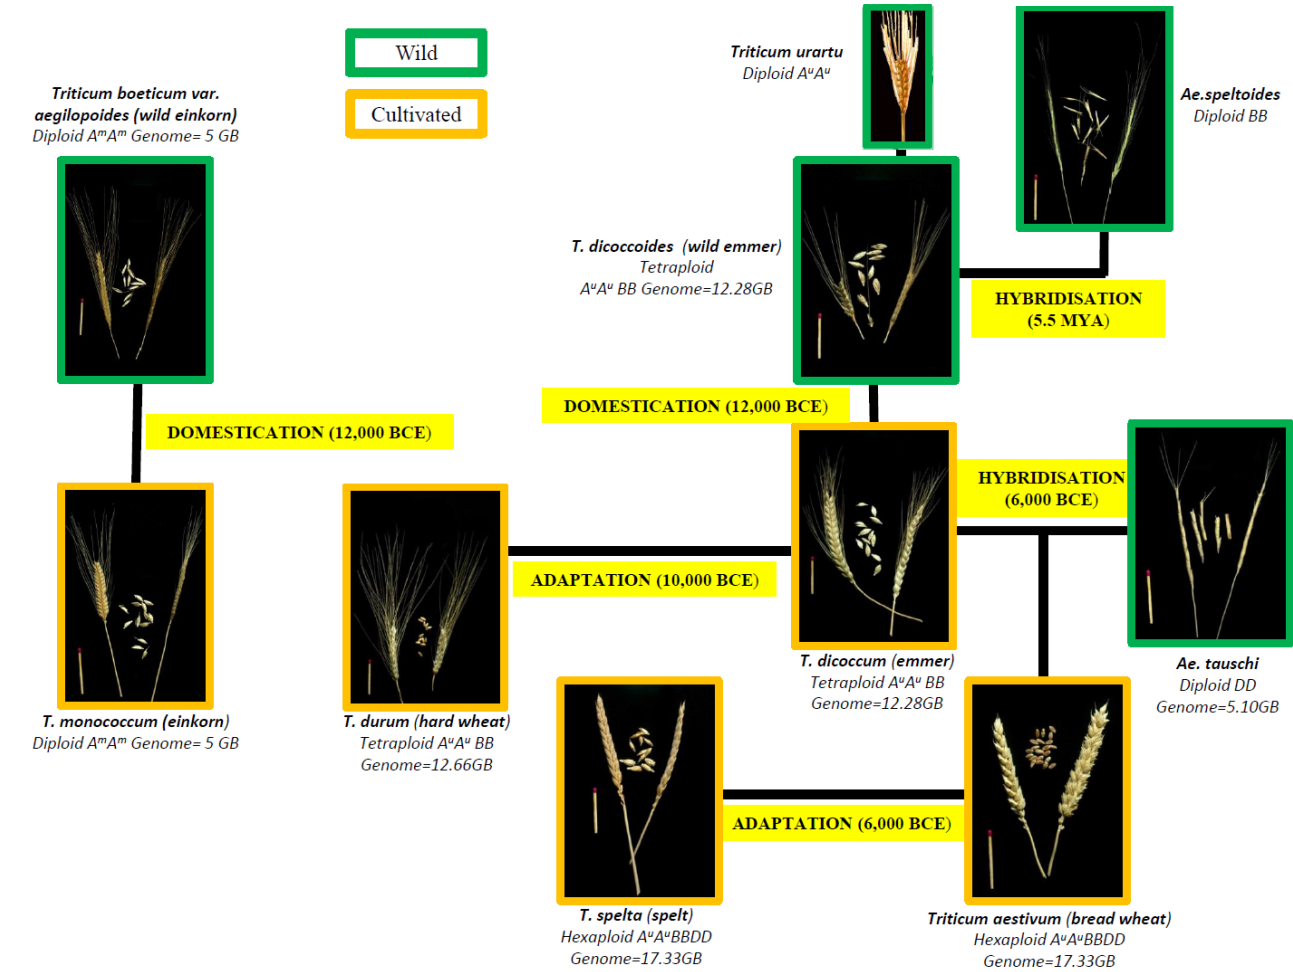
\includegraphics[width=7cm]{./images/philotree.png}
\caption{\label{fig:orgb585cef}
Phylogeny of wheat genotypes (Provided by Dr. Hugo Oliveira)}
\end{figure}
\end{frame}

\begin{frame}[label={sec:orgb5d2bb9}]{Research Question:}
\begin{block}{Is it possible to use \textmu{CT} imaging to answer questions about Wheat domestication?}
\emph{I hope so!}
\end{block}
\begin{block}{Main Groups that we are comparing}
\begin{enumerate}
\item Einkorn Wild and Einkorn Domesticated
\item Emmer Wild and Emmer Domesticated
\item Spelt and Bread wheat
\item Emmer Domesticated and Pasta Wheat
\item Einkorn Wild and Emmer Wild
\end{enumerate}
\end{block}
\end{frame}


\begin{frame}[label={sec:orgfaebbff}]{Aims}
\begin{block}{Primary Aims}
I am wanting to produce:

\begin{itemize}
\item A software library (in Python) which can be used to help analysis of \textmu{CT} scanned seeds
\item A GUI application for researchers to use to auto analyse seeds
\item Descriptions of the differences/similarities of the aforementioned groups
\end{itemize}
\end{block}
\end{frame}


\begin{frame}[label={sec:orgbe02cf8}]{Extracted Features}
\begin{columns}
\begin{column}{0.45\columnwidth}
\begin{block}{Features List}
The features I am collecting are:

\begin{itemize}
\item Length
\item Width
\item Depth
\item Volume
\item Surface Area
\item X,Y,Z coordinates of grains
\end{itemize}
\end{block}
\end{column}

\begin{column}{0.6\columnwidth}
\begin{figure}[htbp]
\centering
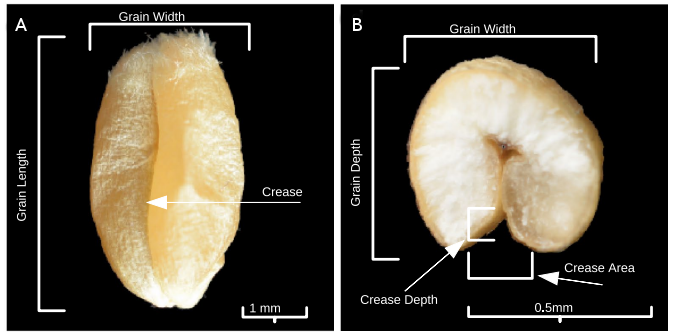
\includegraphics[width=8cm]{./images/seeds.png}
\caption{Major features extracted from analysis}
\end{figure}
\end{column}
\end{columns}
\end{frame}

\section{Materials and Methods}
\label{sec:org910cc87}

\begin{frame}[label={sec:orgfd9c907}]{Materials (Plant)}
\begin{columns}
\begin{column}{0.4\columnwidth}
\begin{block}{Wheat information}
We have a wide range of Wheat genotypes, these are:
\begin{itemize}
\item Ranged between diploid, tetraploid and hexaploid
\item 12 total genotypes
\item Divided between domestication status
\end{itemize}
\end{block}
\end{column}

\begin{column}{0.6\columnwidth}
\vspace{-1.7cm}
\begin{figure}[htbp]
\centering
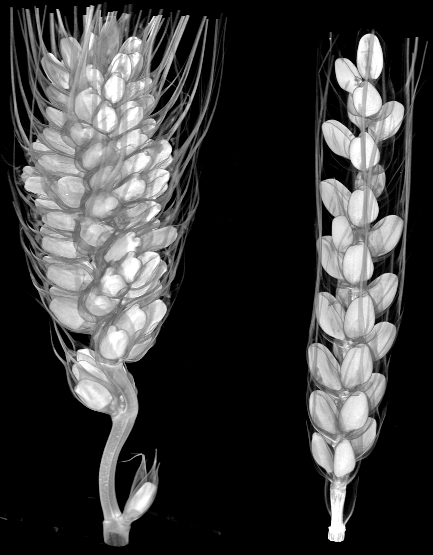
\includegraphics[width=4.6cm]{./images/spikes.png}
\caption{Two wheat spikes, showing diversity in Population, Club Wheat (6N) left, Pasta Wheat right (4N)}
\end{figure}
\end{column}
\end{columns}
\end{frame}

\begin{frame}[label={sec:org0d31c02}]{Methods}
\begin{columns}
\begin{column}{0.5\columnwidth}
\begin{block}{CT Scanning software}
The features where extracted using an improved and optimised version of
our software which was used in our previous study.

\vspace{0.5cm}

Modifications were implemented to handle the wide range of diversity in the population of
this experiment
\end{block}
\end{column}

\begin{column}{0.5\columnwidth}
\vspace{-1cm}
\begin{figure}[htbp]
\centering
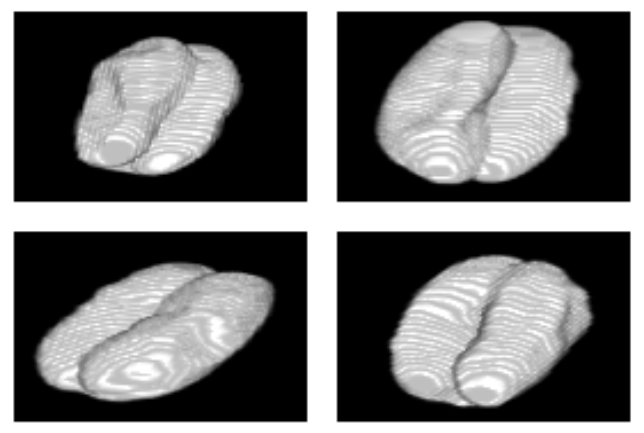
\includegraphics[width=7cm]{./images/ctgrains.png}
\caption{Grains extracted from our imaging software and displayed in 3D}
\end{figure}
\end{column}
\end{columns}
\end{frame}

\section{Data Analysis}
\label{sec:orgddc23e9}
\begin{frame}[label={sec:orgb5bf783}]{Why I don't trust the T-Test}
\begin{block}{Proof of deception}
\begin{figure}[htbp]
\centering
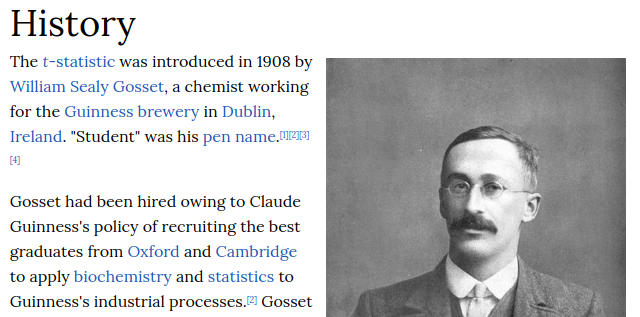
\includegraphics[width=7cm]{./images/ttest.png}
\caption{\label{fig:org7d5b355}
Exhibit A - Why the T-Test is evil}
\end{figure}
\end{block}
\end{frame}

\begin{frame}[label={sec:orgef9cd50}]{Bayesian Hypothesis Testing}
\begin{block}{Why?}
\begin{itemize}[<+->]
\item "Despite their wide use in scientific journals \ldots{}, statistical  hypothesis tests add very little value to the products of research" - \citep{Johnson1999a}
\item It provides interpretable answers, such as “the true parameter \(\theta\) has a probability of 0.95 of falling in a 95\% credible interval.”
\item Allows for missing data points i.e. where a complete range of data is not possible i.e. ALL OF BIOLOGY
\end{itemize}
\end{block}
\end{frame}

\begin{frame}[label={sec:orga804b35}]{Bayesian Model Used}
\begin{block}{Bayes states that}
\begin{itemize}
\item \(P(A|B) \propto P(B|A) \times P(A)\)
\begin{itemize}
\item The posterior is proportional to the likelihood times the prior
\end{itemize}
\item \(P(mean.1 | sample.1) \propto P(sample.1 | mean.1) \times  P(mean.1)\)
\end{itemize}
\end{block}
\begin{block}{Likelihood is described as}
\begin{itemize}
\item \(y_i^{(g)} \sim T(\nu, \mu, \sigma)\)
\begin{itemize}
\item \(\nu\) (Degrees of freedom) is assumed similar for groups \(g\)
\item \(\mu\) (mean) of groups is assumed the same
\item \(\sigma\) (S.D.) is assumed the same
\end{itemize}
\end{itemize}
\end{block}
\end{frame}

\begin{frame}[label={sec:org85e0d5f}]{Prior Mean \(\mu\)}
\begin{columns}
\begin{column}{0.6\columnwidth}
\begin{block}{Mean}
\begin{itemize}
\item Using the method described in \citep{Kruschke2012}
\item \(\mu_k \sim N(\bar{x},2s)\)
\begin{itemize}
\item The data are real-values and normal priors are applied (to ensure the posterior follows suit)
\item \(2s\) - twice the S.D. ensures no values are favoured in the model
\end{itemize}
\end{itemize}
\end{block}
\end{column}

\begin{column}{0.4\columnwidth}
\begin{block}{Distribution}
\begin{figure}[htbp]
\centering
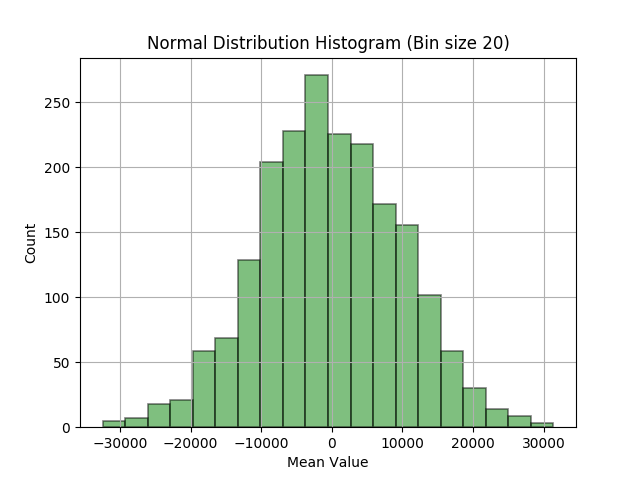
\includegraphics[width=4.5cm]{./images/mu.png}
\caption{\label{fig:org14e0d21}
Normal\((\bar{x},2s)\)}
\end{figure}
\end{block}
\end{column}
\end{columns}
\end{frame}


\begin{frame}[label={sec:org5f2056a}]{Prior Standard Deviations \(\sigma\)}
\begin{columns}
\begin{column}{0.6\columnwidth}
\begin{block}{Standard Deviations}
\begin{itemize}
\item Using the method described in \citep{Kruschke2012}
\item \(\text{Uniform}(1,10000)\) is used
\item Whilst no values in the model will have this range, it makes no difference due to random sampling
\item Figure:\ref{fig:orgd2ed836} shows the distribution expected by random sampling
\end{itemize}
\end{block}
\end{column}
\begin{column}{0.4\columnwidth}
\begin{block}{Distribution}
\begin{figure}[htbp]
\centering
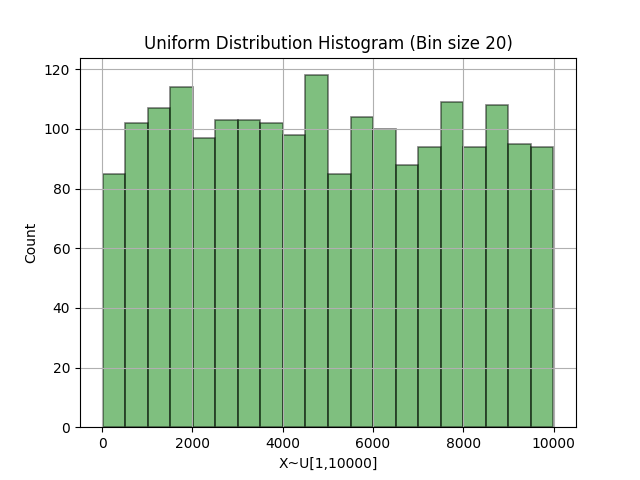
\includegraphics[width=4.5cm]{./images/dist.png}
\caption{\label{fig:orgd2ed836}
Uniform(1,10000)}
\end{figure}
\end{block}
\end{column}
\end{columns}
\end{frame}

\begin{frame}[label={sec:org6170e12}]{Prior Degrees of freedom \(\nu\)}
\begin{columns}
\begin{column}{0.6\columnwidth}
\begin{block}{Degrees of freedom}
\begin{itemize}
\item Using the method described in \citep{Kruschke2012}
\item \(\nu\) of 30 is used with an exponential distribution
\item Shown in Figure:\ref{fig:org280a4cf}
\end{itemize}
\end{block}
\end{column}


\begin{column}{0.4\columnwidth}
\begin{block}{Distribution}
\begin{figure}[htbp]
\centering
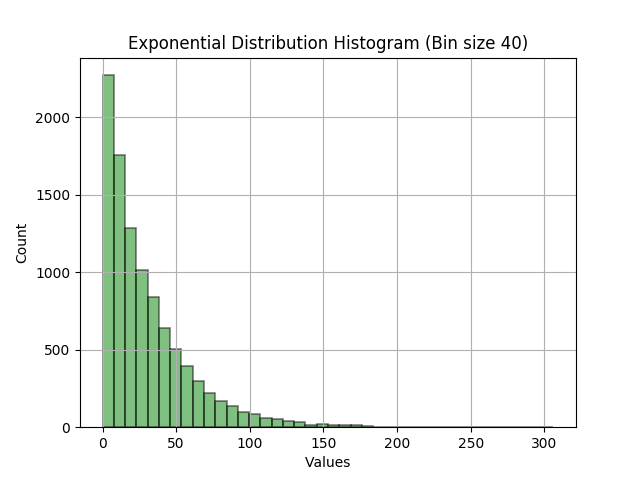
\includegraphics[width=4.5cm]{./images/dist2.png}
\caption{\label{fig:org280a4cf}
Exponential Distribution}
\end{figure}
\end{block}
\end{column}
\end{columns}
\end{frame}



\begin{frame}[label={sec:org7cb6d62}]{Sampling and Testing}
\begin{block}{Markov chain Monte Carlo}
\begin{itemize}
\item 1000 random samples are drawn using Markov chain Monte Carlo
\begin{itemize}
\item This is done twice, independently to ensure convergence of randomness
\end{itemize}
\item These provide a posterior of possibilities where the same mean could exist for the given data
\end{itemize}
\end{block}
\end{frame}

\section{Example of Method}
\label{sec:orgdbf6bd7}
\begin{frame}[label={sec:org5de2bc0}]{Example Input Data}
\begin{figure}[htbp]
\centering
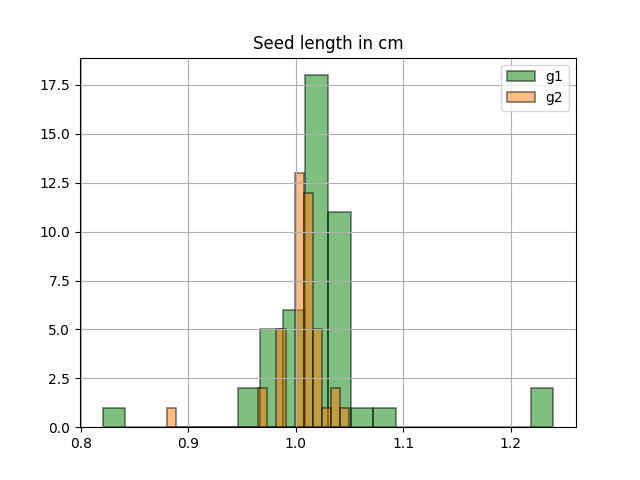
\includegraphics[width=7.5cm]{exampledata.png}
\caption{\label{fig:orga0f27eb}
Histogram of input data}
\end{figure}
\end{frame}

\begin{frame}[label={sec:org51e811f}]{Example Posterior}
\begin{figure}[htbp]
\centering
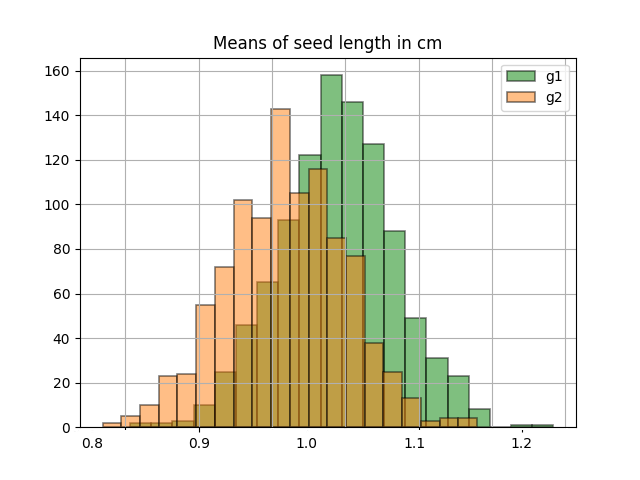
\includegraphics[width=7.5cm]{examplebayes.png}
\caption{\label{fig:orgc2bd539}
Histogram of posterior data}
\end{figure}
\end{frame}

\begin{frame}[label={sec:orgc7e5336}]{Example Difference of Means}
\begin{figure}[htbp]
\centering
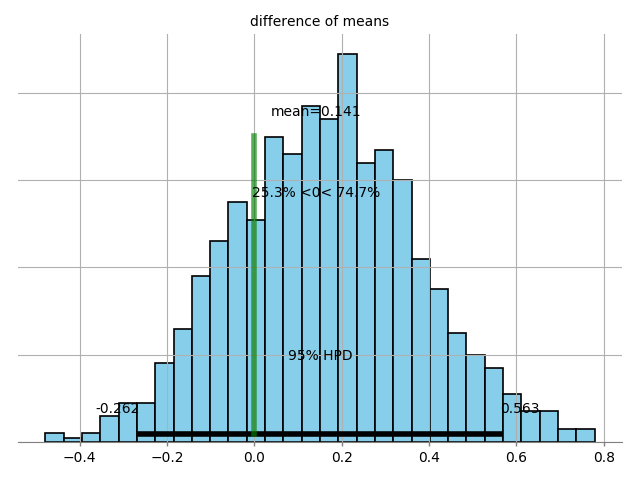
\includegraphics[width=7.5cm]{examplebayes2.png}
\caption{\label{fig:org91985a6}
Histogram of posterior data subtracted}
\end{figure}
\end{frame}

\begin{frame}[label={sec:org84672a1}]{Example Forest Plot}
\begin{figure}[htbp]
\centering
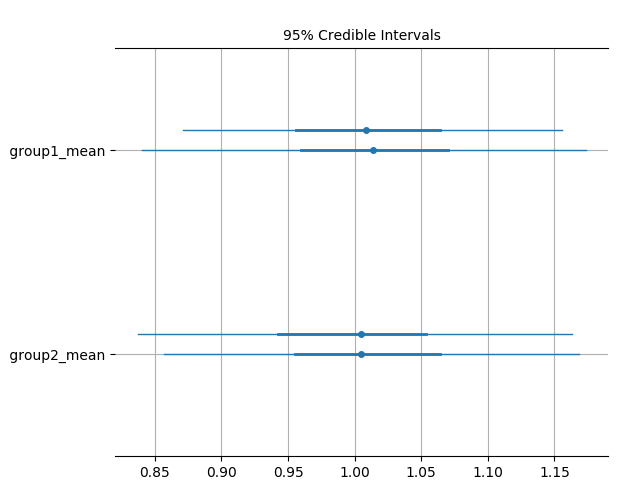
\includegraphics[width=7.5cm]{examplebayes3.png}
\caption{\label{fig:orgaa1a50c}
Forest Plot of both chains (bold is 95\% of data)}
\end{figure}
\end{frame}

\section{Results}
\label{sec:org58ad5a3}

\begin{frame}[label={sec:orgf0bf5f1}]{Einkorn Wild and Einkorn Domesticate (\(P<0.01\))}
\begin{columns}
\begin{column}{0.5\columnwidth}
\begin{block}{Boxplots}
\begin{figure}[htbp]
\centering
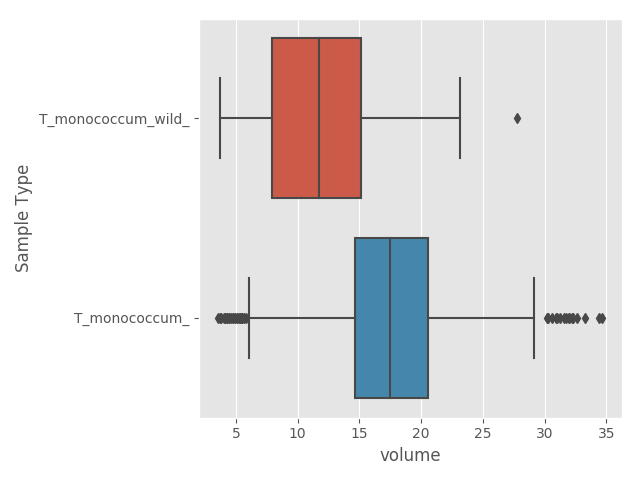
\includegraphics[width=4.5cm]{./images/monobox.png}
\caption{\label{fig:org9ac8b37}
Boxplot for volume}
\end{figure}
\end{block}
\end{column}

\begin{column}{0.5\columnwidth}
\begin{block}{Difference of means}
\begin{figure}[htbp]
\centering
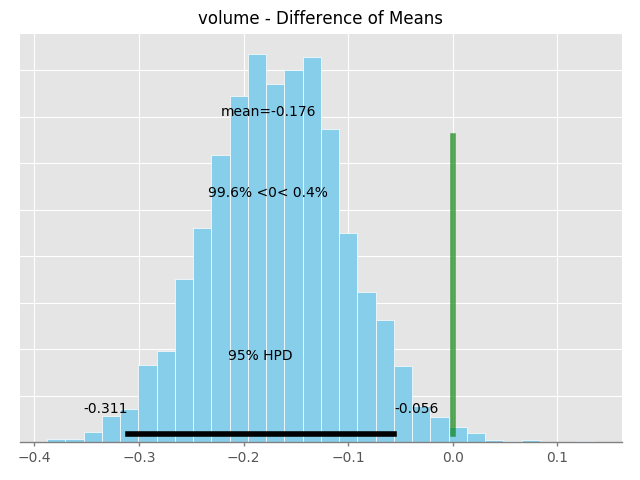
\includegraphics[width=4.5cm]{./images/monodiff.png}
\caption{\label{fig:org257fc30}
Difference of means}
\end{figure}
\end{block}
\end{column}
\end{columns}
\end{frame}


\begin{frame}[label={sec:org7c5fc2c}]{Emmer Wild and Emmer Domesticated (\(P = 0.032\))}
\begin{columns}
\begin{column}{0.5\columnwidth}
\begin{block}{Boxplots}
\begin{figure}[htbp]
\centering
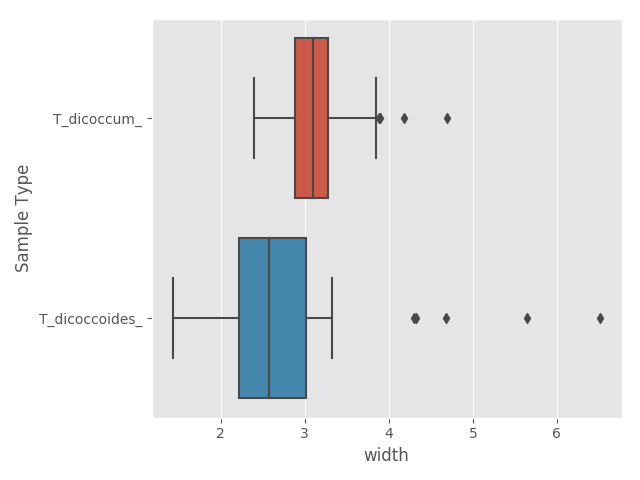
\includegraphics[width=4.5cm]{./images/dicbox.png}
\caption{\label{fig:orgdacaa5b}
Boxplot for width}
\end{figure}
\end{block}
\end{column}

\begin{column}{0.5\columnwidth}
\begin{block}{Difference of means}
\begin{figure}[htbp]
\centering
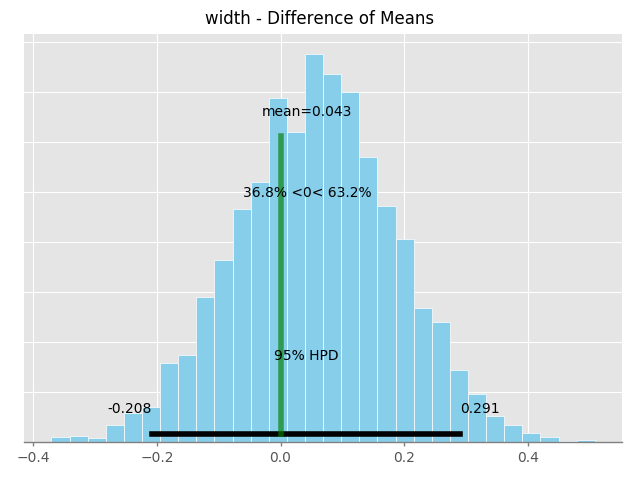
\includegraphics[width=4.5cm]{./images/dicdiff.png}
\caption{\label{fig:org9a7ed8e}
Difference of means}
\end{figure}
\end{block}
\end{column}
\end{columns}
\end{frame}



\begin{frame}[label={sec:org67c4da6}]{Spelt and Bread wheat (\(P = 0.11\))}
\begin{columns}
\begin{column}{0.5\columnwidth}
\begin{block}{Boxplots}
\begin{figure}[htbp]
\centering
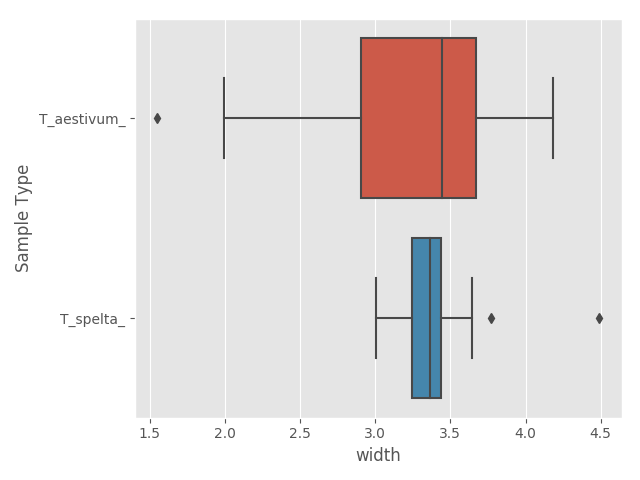
\includegraphics[width=4.5cm]{./images/speltbox.png}
\caption{\label{fig:org3325aa4}
Boxplot for width}
\end{figure}
\end{block}
\end{column}

\begin{column}{0.5\columnwidth}
\begin{block}{Difference of means}
\begin{figure}[htbp]
\centering
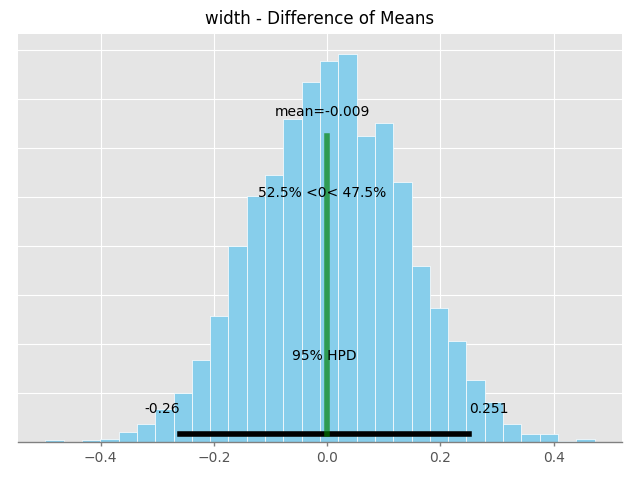
\includegraphics[width=4.5cm]{./images/speltdiff.png}
\caption{\label{fig:orge07c859}
Difference of means}
\end{figure}
\end{block}
\end{column}
\end{columns}
\end{frame}




\section{Software Progress}
\label{sec:org2d007b1}

\begin{frame}[label={sec:org755d612}]{Loading CT Data}
\begin{figure}[htbp]
\centering
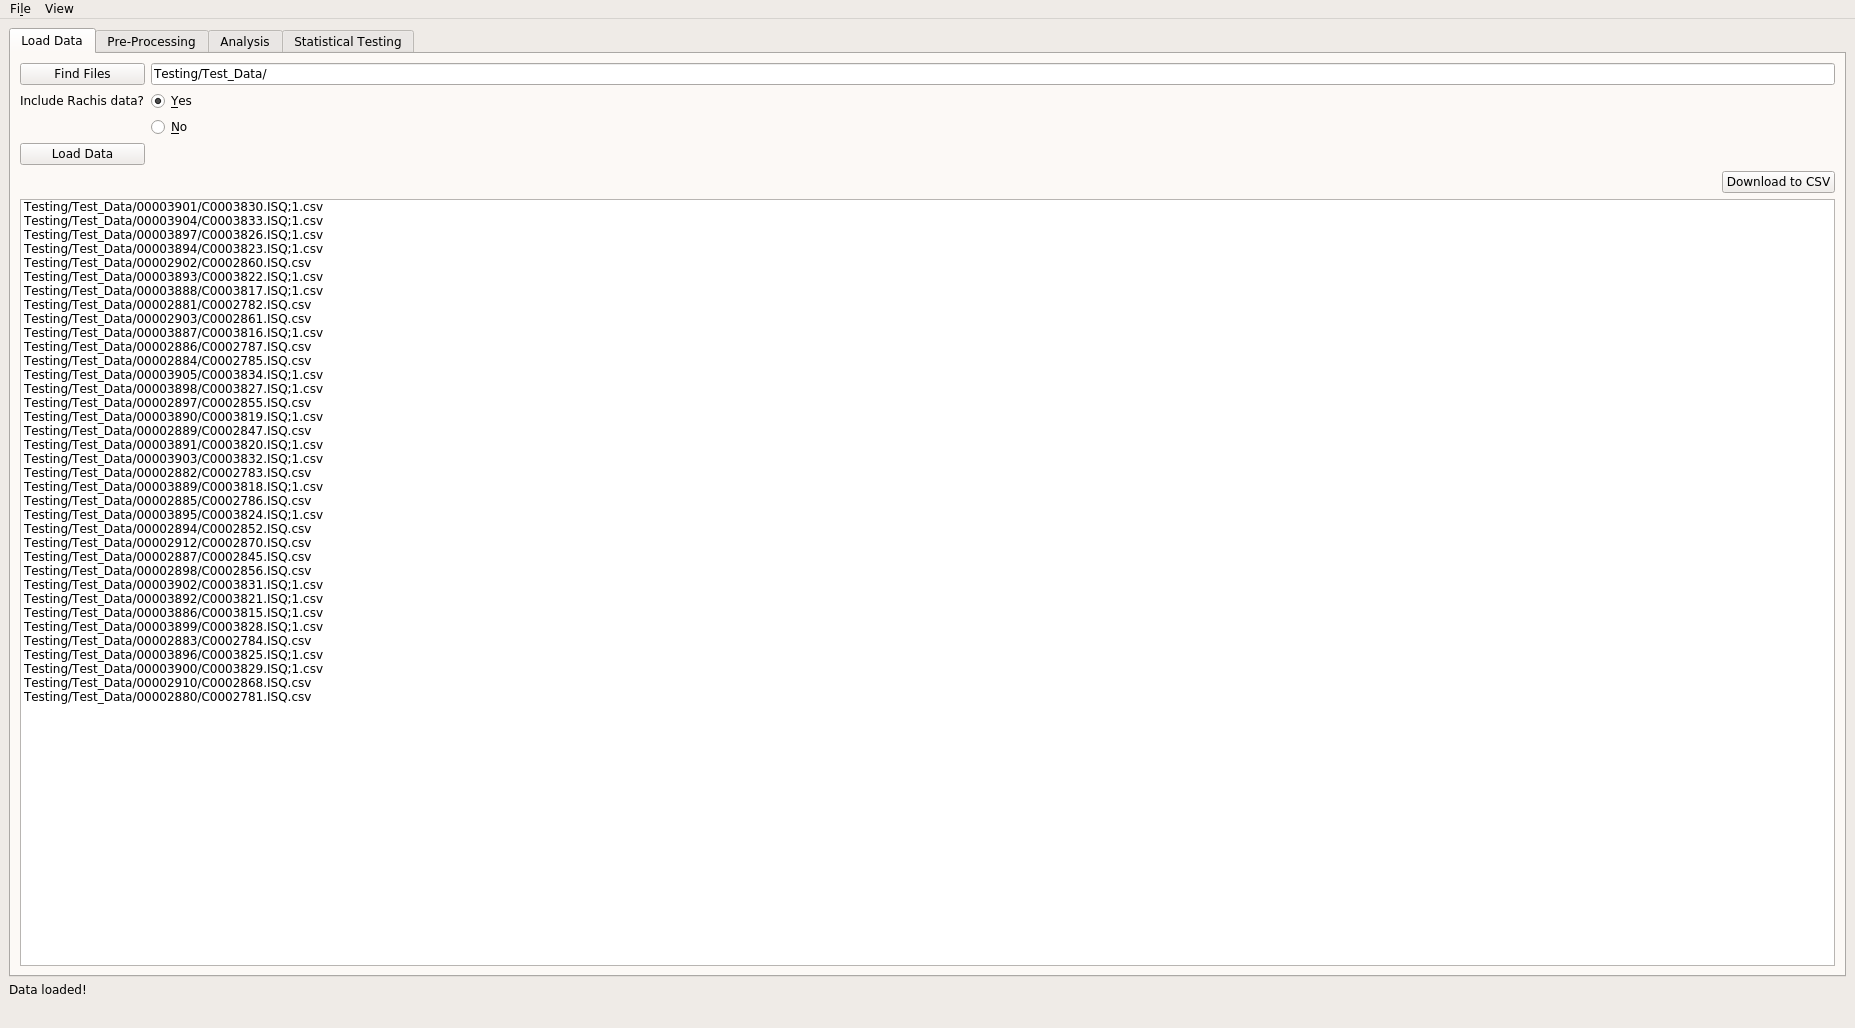
\includegraphics[width=10cm]{./images/1.png}
\caption{\label{fig:org48a1774}
Showing the Data loading window}
\end{figure}
\end{frame}

\begin{frame}[label={sec:orgb622236}]{Investigating CT Data Distributions}
\begin{figure}[htbp]
\centering
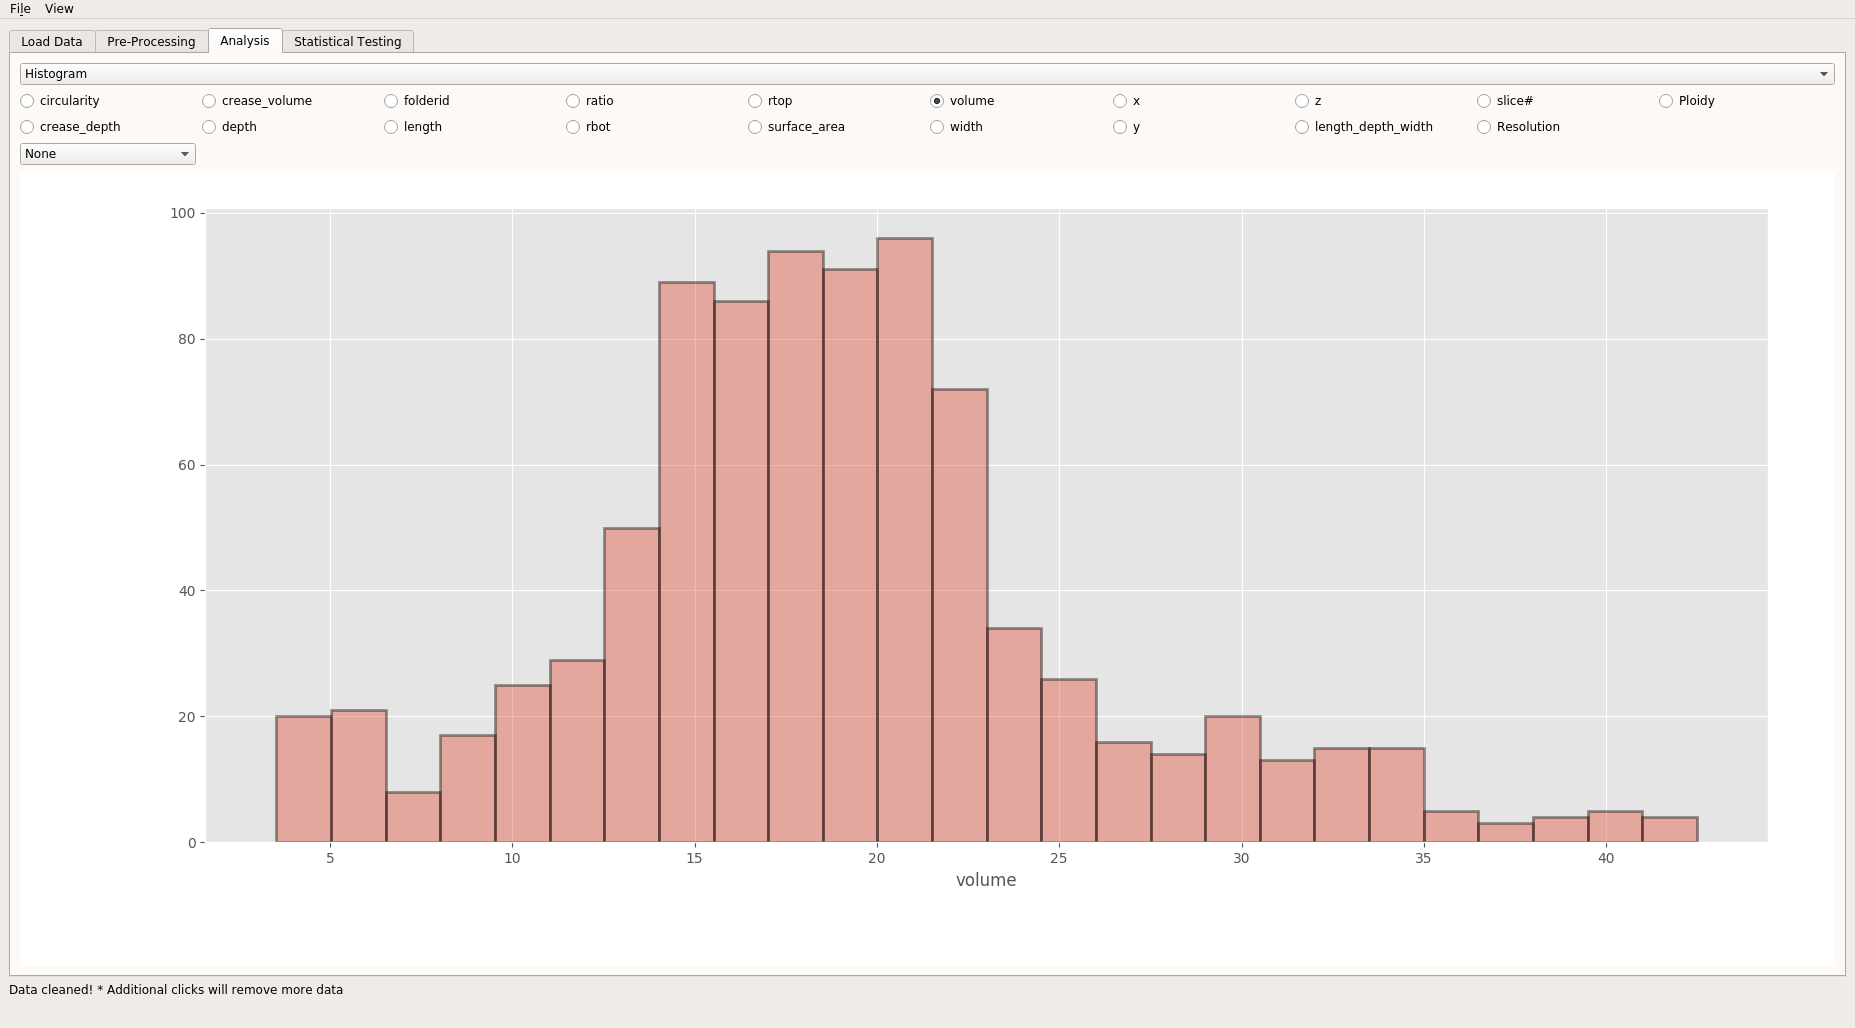
\includegraphics[width=10cm]{./images/2.png}
\caption{\label{fig:orgaa71575}
Histogram of some data attributes}
\end{figure}
\end{frame}


\begin{frame}[label={sec:org3c5e783}]{Comparing CT Data Distributions}
\begin{figure}[htbp]
\centering
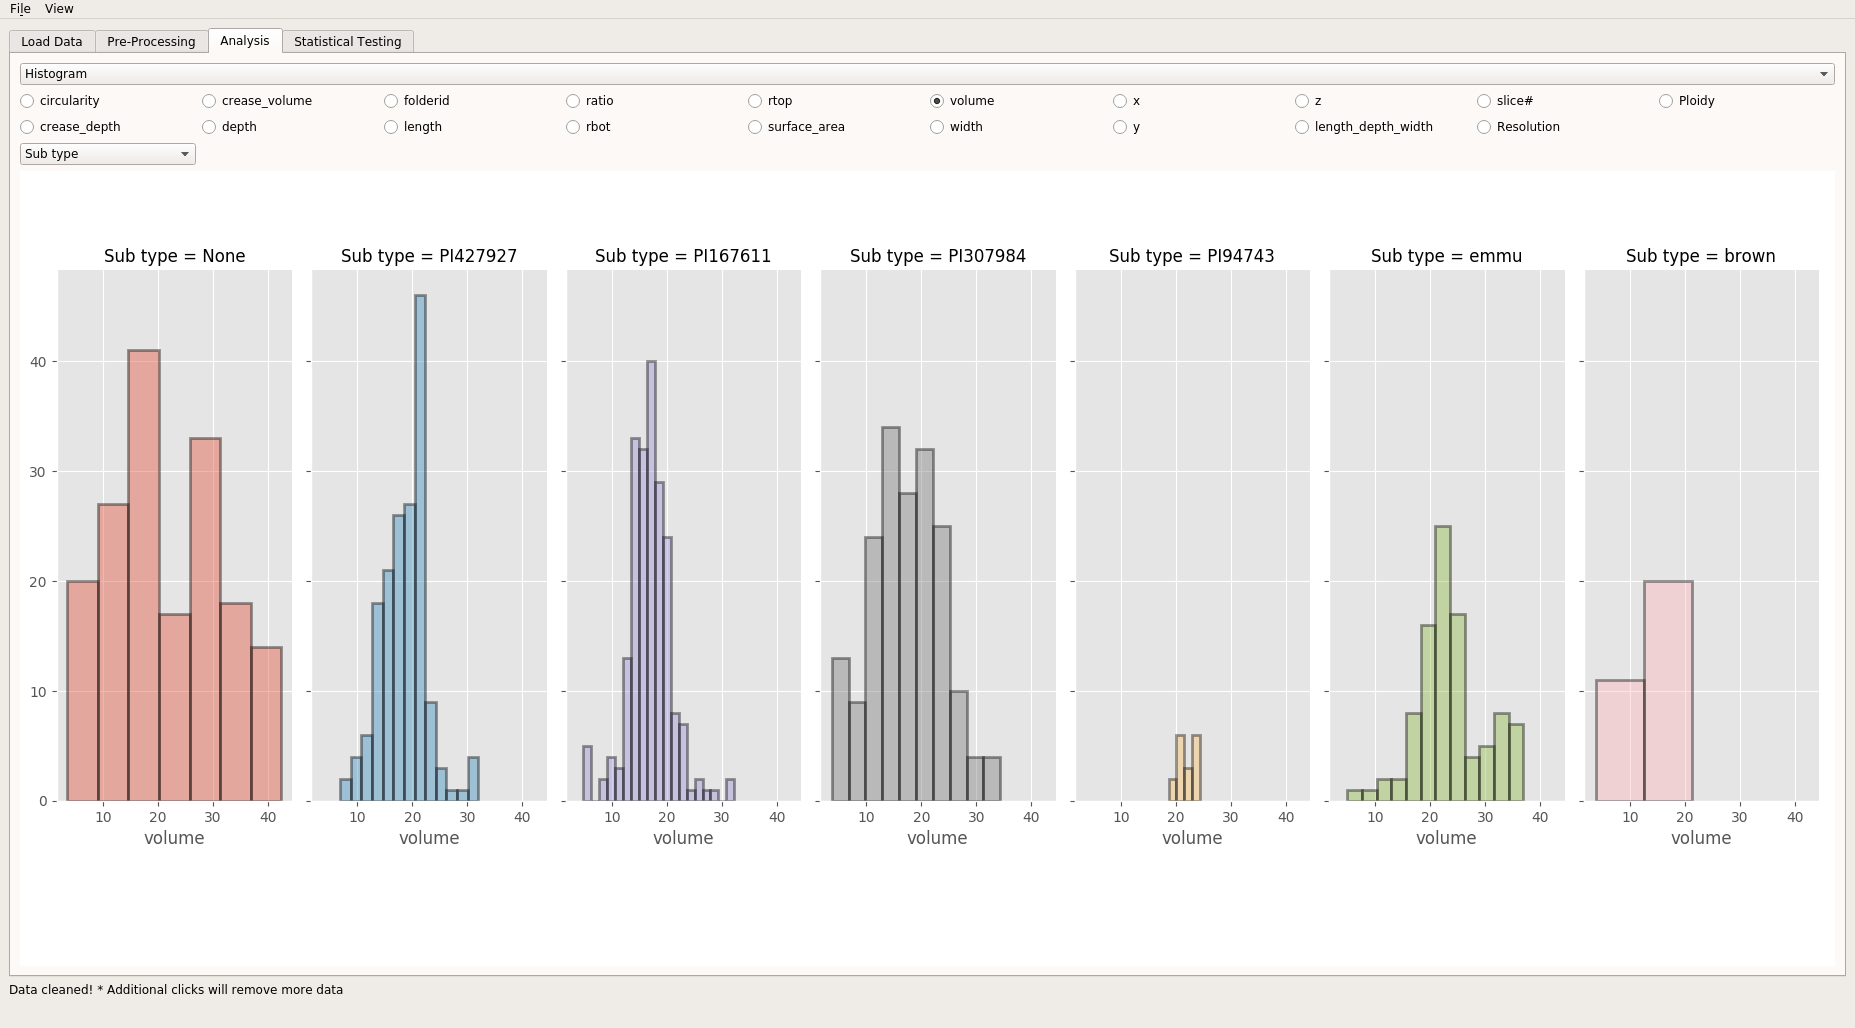
\includegraphics[width=10cm]{./images/3.png}
\caption{\label{fig:org2c58578}
Grouping by data columns}
\end{figure}
\end{frame}


\begin{frame}[label={sec:org7449267}]{Running T-Tests on CT Data}
\begin{figure}[htbp]
\centering
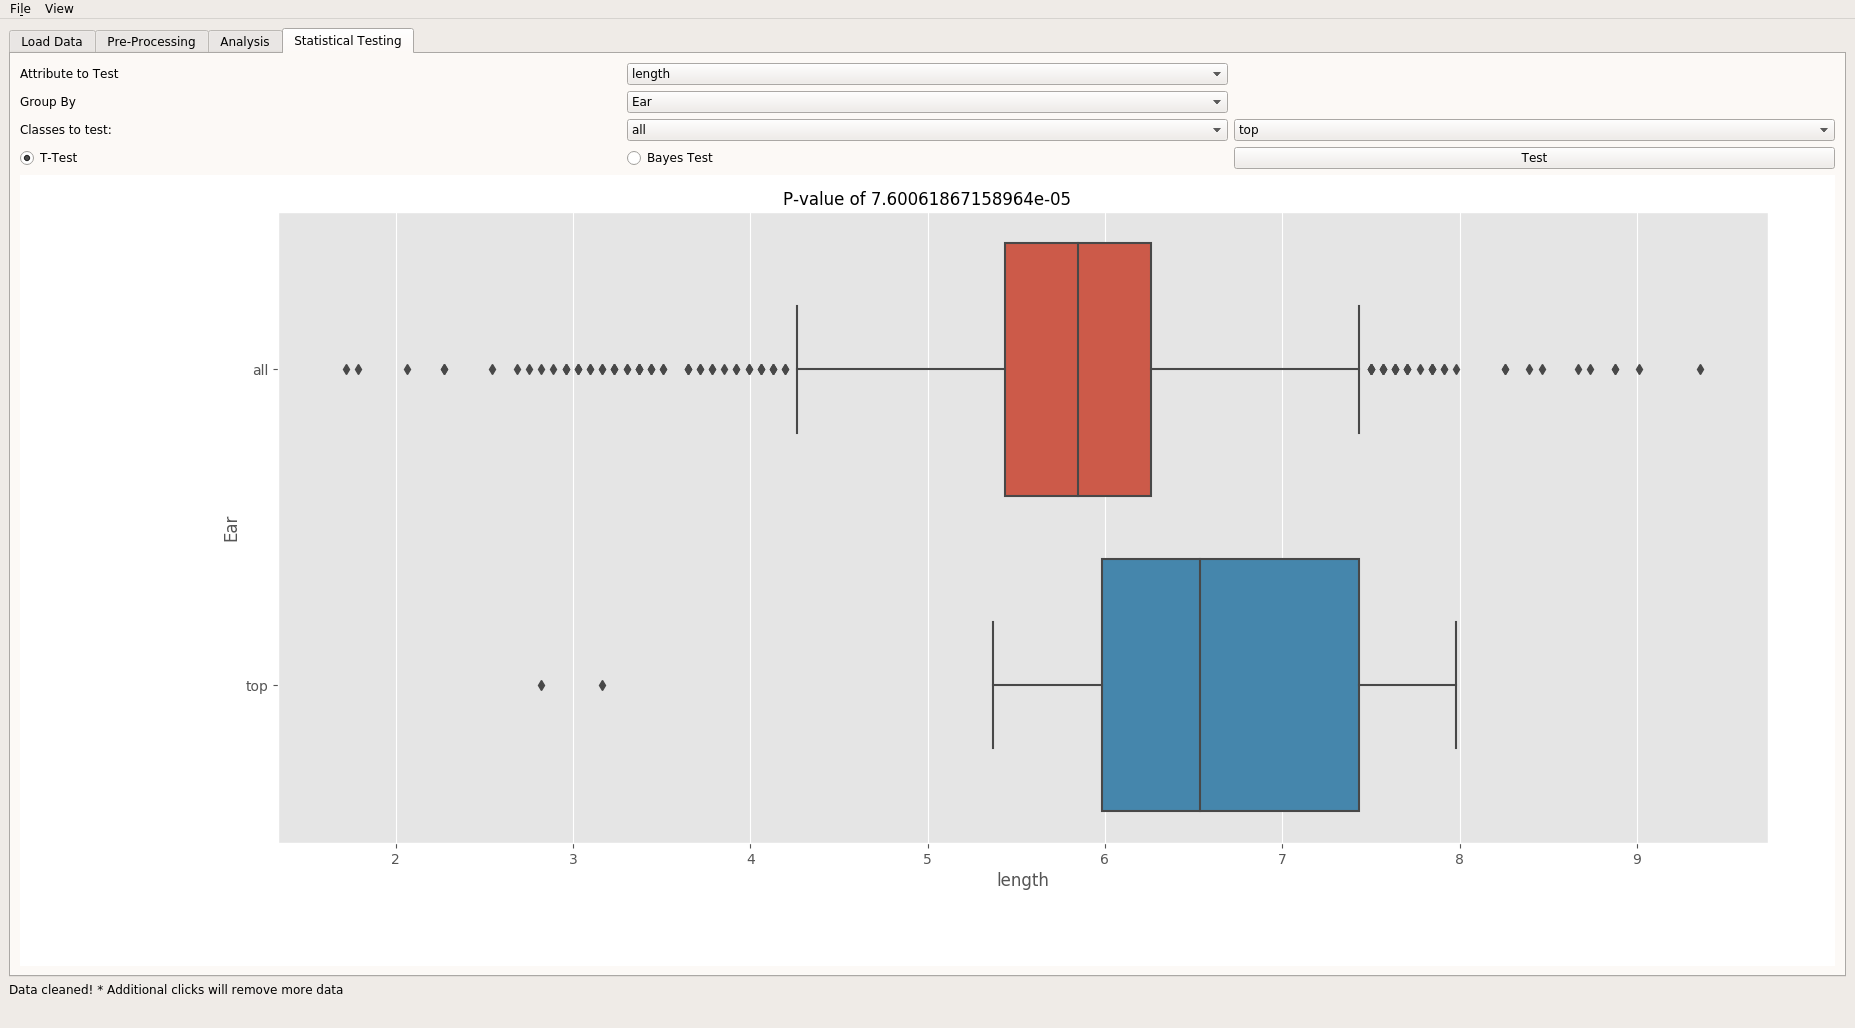
\includegraphics[width=10cm]{./images/4.png}
\caption{\label{fig:org4ed12a0}
Running T-Tests}
\end{figure}
\end{frame}


\begin{frame}[label={sec:org5433df0}]{Running Bayesian Tests on CT Data}
\begin{figure}[htbp]
\centering
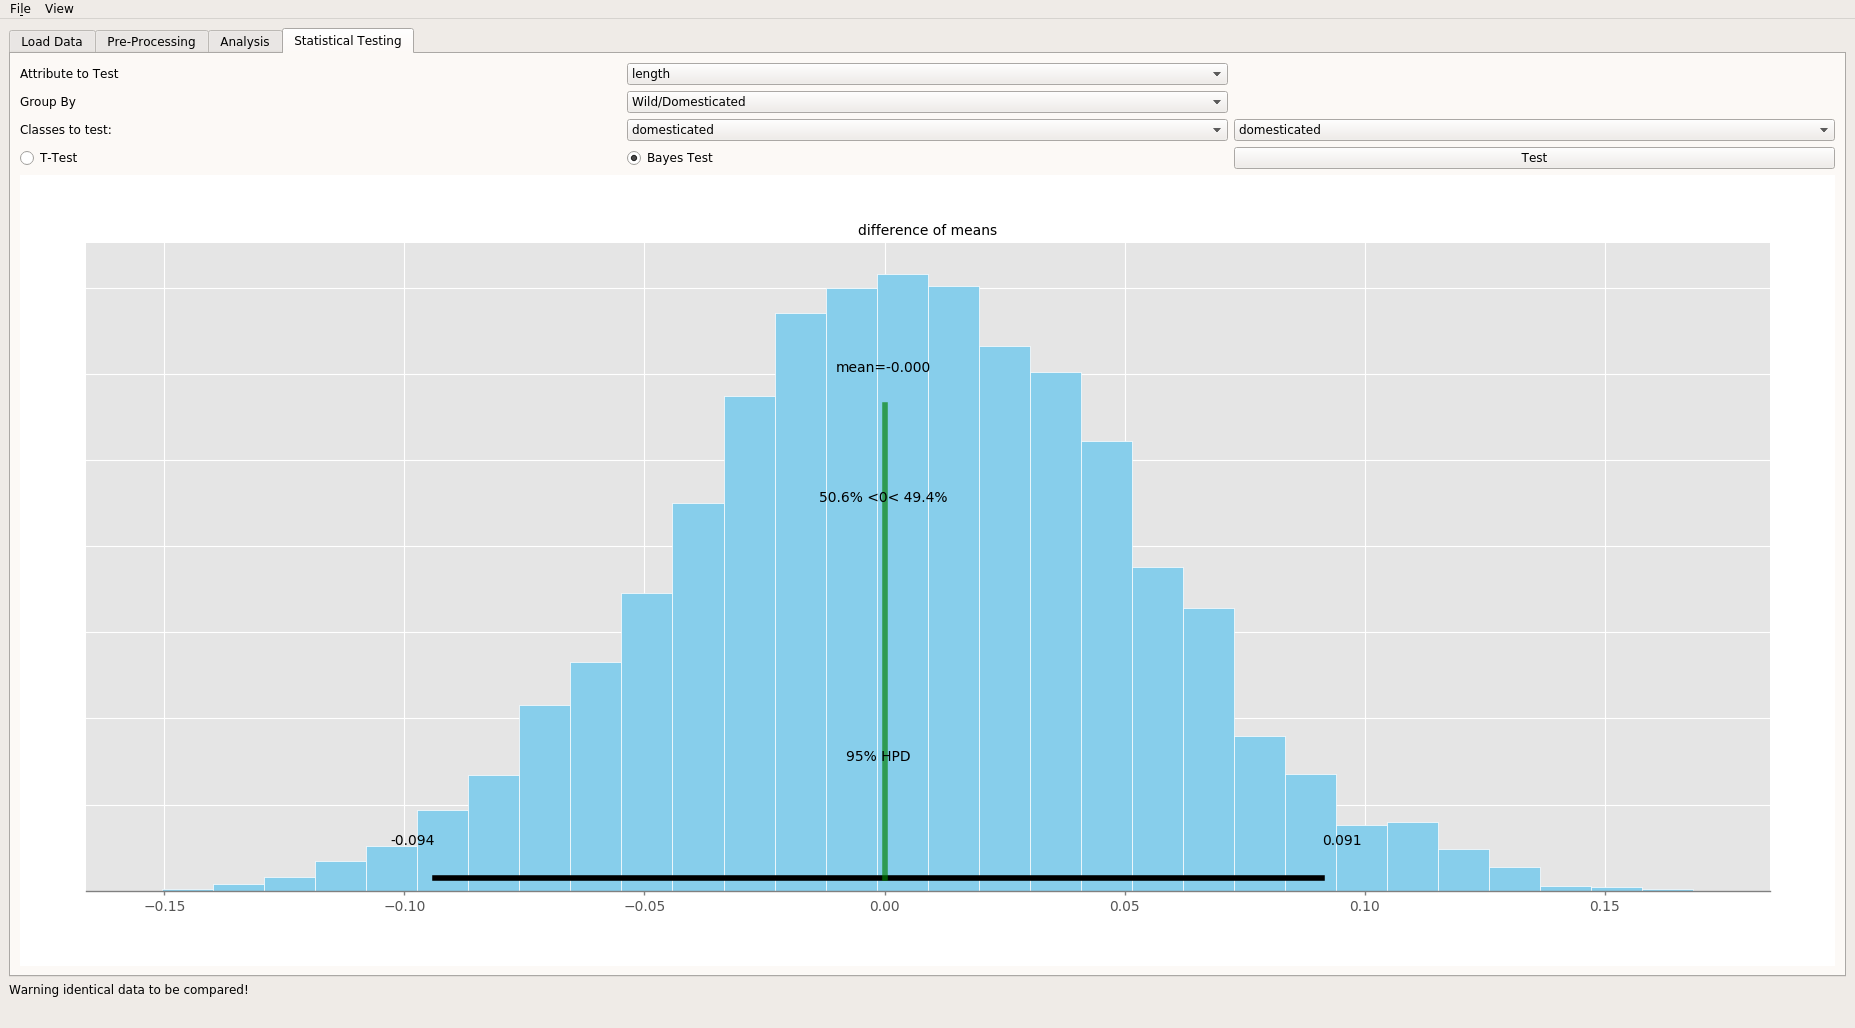
\includegraphics[width=10cm]{./images/5.png}
\caption{\label{fig:org0e15725}
Running Bayesian Tests}
\end{figure}
\end{frame}



\section{Thanks}
\label{sec:org259b02d}

\begin{frame}[label={sec:orgfcf627f}]{Thanks to}
\begin{block}{All these people:}
\begin{longtable}{ll}
\label{tab:orge599cb2}
\\
Dr. Wayne Aubrey & Prof. John Doonan\\
Dr. Candida Nibau & Dr. Kevin Williams\\
Mr. Jason Brook & Everyone at the NPPC\\
\end{longtable}
\end{block}
\end{frame}
\begin{frame}[label={sec:org0267e39}]{References}
\bibliography{library}
\bibliographystyle{plainnat}
\end{frame}
\end{document}
